\section{System's perspective} \label{section:System perspective}
\todo{argue for the choice of technologies and decisions for at least all cases for which we asked you to do so in the tasks at the end of each session.}
\subsection{Design} %Jonas

\subsection{Architecture} %Jonas

\subsection{Dependencies } %Nikolaj %god ide med license her
\begin{itemize}
    \item \textbf{Spark Java}:A micro framework for creating web applications with minimal effort. Suitable for the minitwit project size and gave us the freedom to structure the application how we wanted it.
    \item \textbf{jinjava}: template engine based on django template syntax, used to render jinja templates. Chosen to mimic the python minitwit with minimal effort. 
    \item \textbf{PicoContainer}: General purpose IoC container.
    \item \textbf{NORM}: Lightweight ORM that doesn't require the complex markdown files that Hibernate, JPA etc. introduce. Suitable for smaller projects with simple models. 
    \item \textbf{MySQL}: Relational database. Chosen based on familiarity to team members and it's renowned reliability for how long it's been around.  
    \item \textbf{JUnit 5}: Most popular unit-testing framework.
    \item \textbf{Mockito}: Mocking framework with a simple API.
    \item \textbf{SLF4J}: Logging Facade for ELK stack. 
    \item \textbf{prometheus}: Prometheus JVM Client for introducing instrumenting such as gauges, counters and other metrics.
    \item \textbf{org.json}: Toolkit for JSON.
\end{itemize}
\todo{Skal plugins nævnes?(maven, PMD, forbiddenAPIs) \textcolor{yellow}{Maven kunne måske være relevant i hvert fald}}


We used \url{www.licensediscovery.io} to analyze our Maven dependency licenses. As seen in figure \ref{fig:licenceDep} the strictest license that the majority of dependencies is ruled by is the Apache Software Licence Version 2. This is the license that we therefore went with.\footnote{\url{https://github.com/DevOps2021-gb/devops2021/blob/main/LICENSE.md}} \todo{Er det begrundelse nok?}
\begin{figure}[!htb]
    \centering
    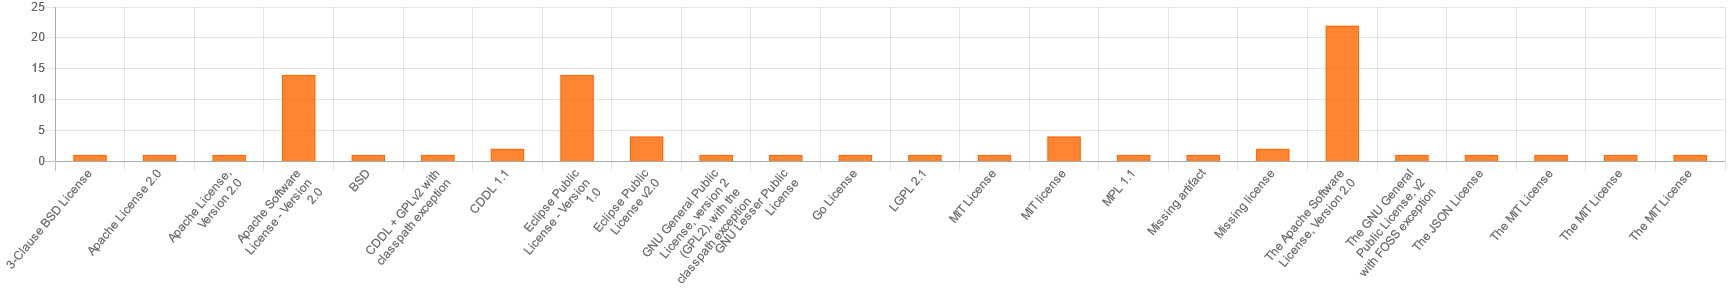
\includegraphics[scale=0.2]{LicenceDependencies.png}
    \caption{Overview of dependency licenses. Sub-dependencies included.}
    \label{fig:licenceDep}
\end{figure}


\subsection{Important interactions of subsystem}

\subsection{Current state of system}
The system is currently has a single known bug regarding the scaling of the system, see section \ref{issues-operation}. The tool used for static analysis, \texttt{sonarcloud}, reports the best rating, \textit{A}, on all measures, with 

\begin{itemize}
    \item 0 bugs
    \item 0 code vulnerabilities and 0 security hotspots
    \item 6 hours code debt due to 63 code smells
    \item 0.0\% code duplication and 0 duplicated blocks
\end{itemize}

Out of the 63 code smells only 11 are major, critical or blockers and all 63 has been assessed as issues that can ignored.

